% Created by tikzDevice version 0.11 on 2018-04-09 17:29:02
% !TEX encoding = UTF-8 Unicode
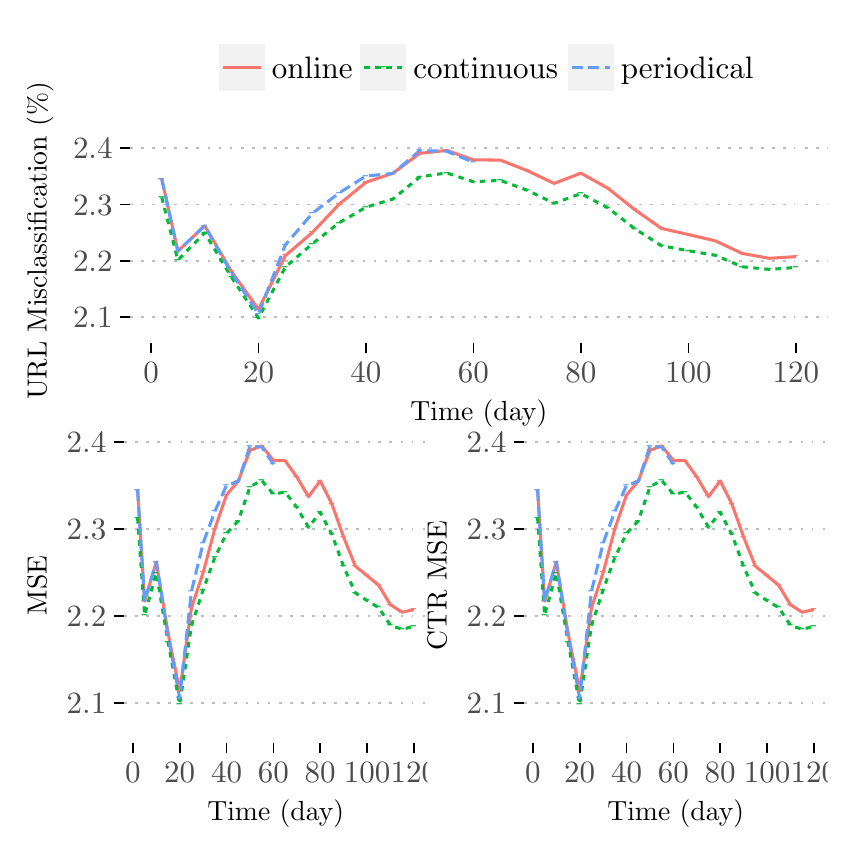
\begin{tikzpicture}[x=1pt,y=1pt]
\definecolor{fillColor}{RGB}{255,255,255}
\path[use as bounding box,fill=fillColor,fill opacity=0.00] (0,0) rectangle (289.08,289.08);
\begin{scope}
\path[clip] (  0.00,144.54) rectangle (289.08,289.08);
\definecolor{drawColor}{RGB}{255,255,255}
\definecolor{fillColor}{RGB}{255,255,255}

\path[draw=drawColor,line width= 0.6pt,line join=round,line cap=round,fill=fillColor] (  0.00,144.54) rectangle (289.08,289.08);
\end{scope}
\begin{scope}
\path[clip] ( 36.99,175.02) rectangle (289.08,248.97);
\definecolor{fillColor}{RGB}{255,255,255}

\path[fill=fillColor] ( 36.99,175.02) rectangle (289.08,248.97);
\definecolor{drawColor}{RGB}{255,255,255}

\path[draw=drawColor,line width= 0.3pt,line join=round] ( 36.99,194.68) --
	(289.08,194.68);

\path[draw=drawColor,line width= 0.3pt,line join=round] ( 36.99,215.05) --
	(289.08,215.05);

\path[draw=drawColor,line width= 0.3pt,line join=round] ( 36.99,235.42) --
	(289.08,235.42);

\path[draw=drawColor,line width= 0.3pt,line join=round] ( 63.99,175.02) --
	( 63.99,248.97);

\path[draw=drawColor,line width= 0.3pt,line join=round] (102.83,175.02) --
	(102.83,248.97);

\path[draw=drawColor,line width= 0.3pt,line join=round] (141.67,175.02) --
	(141.67,248.97);

\path[draw=drawColor,line width= 0.3pt,line join=round] (180.51,175.02) --
	(180.51,248.97);

\path[draw=drawColor,line width= 0.3pt,line join=round] (219.36,175.02) --
	(219.36,248.97);

\path[draw=drawColor,line width= 0.3pt,line join=round] (258.20,175.02) --
	(258.20,248.97);
\definecolor{drawColor}{RGB}{190,190,190}

\path[draw=drawColor,line width= 0.6pt,dash pattern=on 1pt off 3pt ,line join=round] ( 36.99,184.49) --
	(289.08,184.49);

\path[draw=drawColor,line width= 0.6pt,dash pattern=on 1pt off 3pt ,line join=round] ( 36.99,204.87) --
	(289.08,204.87);

\path[draw=drawColor,line width= 0.6pt,dash pattern=on 1pt off 3pt ,line join=round] ( 36.99,225.24) --
	(289.08,225.24);

\path[draw=drawColor,line width= 0.6pt,dash pattern=on 1pt off 3pt ,line join=round] ( 36.99,245.61) --
	(289.08,245.61);
\definecolor{drawColor}{RGB}{255,255,255}

\path[draw=drawColor,line width= 0.6pt,line join=round] ( 44.58,175.02) --
	( 44.58,248.97);

\path[draw=drawColor,line width= 0.6pt,line join=round] ( 83.41,175.02) --
	( 83.41,248.97);

\path[draw=drawColor,line width= 0.6pt,line join=round] (122.25,175.02) --
	(122.25,248.97);

\path[draw=drawColor,line width= 0.6pt,line join=round] (161.09,175.02) --
	(161.09,248.97);

\path[draw=drawColor,line width= 0.6pt,line join=round] (199.94,175.02) --
	(199.94,248.97);

\path[draw=drawColor,line width= 0.6pt,line join=round] (238.78,175.02) --
	(238.78,248.97);

\path[draw=drawColor,line width= 0.6pt,line join=round] (277.62,175.02) --
	(277.62,248.97);
\definecolor{drawColor}{RGB}{248,118,109}

\path[draw=drawColor,line width= 1.1pt,line join=round] ( 48.45,234.41) --
	( 54.27,208.33) --
	( 63.98,217.50) --
	( 73.69,200.93) --
	( 83.41,187.29) --
	( 93.12,206.70) --
	(102.83,215.02) --
	(112.54,225.27) --
	(122.25,233.21) --
	(131.96,236.47) --
	(141.67,243.66) --
	(151.38,244.72) --
	(161.09,241.31) --
	(170.80,241.23) --
	(180.51,237.43) --
	(190.22,232.81) --
	(199.94,236.49) --
	(209.65,231.08) --
	(219.36,223.34) --
	(229.07,216.53) --
	(238.78,214.31) --
	(248.49,212.05) --
	(258.20,207.49) --
	(267.91,205.74) --
	(277.62,206.34);
\definecolor{drawColor}{RGB}{0,186,56}

\path[draw=drawColor,line width= 1.1pt,dash pattern=on 2pt off 2pt ,line join=round] ( 48.45,227.78) --
	( 54.27,205.07) --
	( 63.98,214.95) --
	( 73.69,198.82) --
	( 83.41,184.14) --
	( 93.12,202.58) --
	(102.83,210.94) --
	(112.54,218.57) --
	(122.25,224.19) --
	(131.96,227.14) --
	(141.67,235.13) --
	(151.38,236.61) --
	(161.09,233.40) --
	(170.80,233.90) --
	(180.51,230.33) --
	(190.22,225.62) --
	(199.94,229.12) --
	(209.65,223.98) --
	(219.36,216.43) --
	(229.07,210.27) --
	(238.78,208.46) --
	(248.49,206.82) --
	(258.20,202.68) --
	(267.91,201.73) --
	(277.62,202.44);
\definecolor{drawColor}{RGB}{97,156,255}

\path[draw=drawColor,line width= 1.1pt,dash pattern=on 4pt off 2pt ,line join=round] ( 48.45,234.41) --
	( 54.27,208.33) --
	( 63.98,217.50) --
	( 73.69,200.32) --
	( 83.41,185.61) --
	( 93.12,210.61) --
	(102.83,221.94) --
	(112.54,229.34) --
	(122.25,235.48) --
	(131.96,236.40) --
	(141.67,244.63) --
	(151.38,244.44) --
	(161.09,240.45);
\definecolor{drawColor}{RGB}{248,118,109}

\node[text=drawColor,anchor=base,inner sep=0pt, outer sep=0pt, scale=  0.72] at ( 48.45,232.86) {-};

\node[text=drawColor,anchor=base,inner sep=0pt, outer sep=0pt, scale=  0.72] at ( 54.27,206.78) {-};

\node[text=drawColor,anchor=base,inner sep=0pt, outer sep=0pt, scale=  0.72] at ( 63.98,215.95) {-};

\node[text=drawColor,anchor=base,inner sep=0pt, outer sep=0pt, scale=  0.72] at ( 73.69,199.38) {-};

\node[text=drawColor,anchor=base,inner sep=0pt, outer sep=0pt, scale=  0.72] at ( 83.41,185.74) {-};

\node[text=drawColor,anchor=base,inner sep=0pt, outer sep=0pt, scale=  0.72] at ( 93.12,205.15) {-};

\node[text=drawColor,anchor=base,inner sep=0pt, outer sep=0pt, scale=  0.72] at (102.83,213.47) {-};

\node[text=drawColor,anchor=base,inner sep=0pt, outer sep=0pt, scale=  0.72] at (112.54,223.72) {-};

\node[text=drawColor,anchor=base,inner sep=0pt, outer sep=0pt, scale=  0.72] at (122.25,231.66) {-};

\node[text=drawColor,anchor=base,inner sep=0pt, outer sep=0pt, scale=  0.72] at (131.96,234.91) {-};

\node[text=drawColor,anchor=base,inner sep=0pt, outer sep=0pt, scale=  0.72] at (141.67,242.10) {-};

\node[text=drawColor,anchor=base,inner sep=0pt, outer sep=0pt, scale=  0.72] at (151.38,243.17) {-};

\node[text=drawColor,anchor=base,inner sep=0pt, outer sep=0pt, scale=  0.72] at (161.09,239.76) {-};

\node[text=drawColor,anchor=base,inner sep=0pt, outer sep=0pt, scale=  0.72] at (170.80,239.68) {-};

\node[text=drawColor,anchor=base,inner sep=0pt, outer sep=0pt, scale=  0.72] at (180.51,235.88) {-};

\node[text=drawColor,anchor=base,inner sep=0pt, outer sep=0pt, scale=  0.72] at (190.22,231.26) {-};

\node[text=drawColor,anchor=base,inner sep=0pt, outer sep=0pt, scale=  0.72] at (199.94,234.94) {-};

\node[text=drawColor,anchor=base,inner sep=0pt, outer sep=0pt, scale=  0.72] at (209.65,229.53) {-};

\node[text=drawColor,anchor=base,inner sep=0pt, outer sep=0pt, scale=  0.72] at (219.36,221.79) {-};

\node[text=drawColor,anchor=base,inner sep=0pt, outer sep=0pt, scale=  0.72] at (229.07,214.98) {-};

\node[text=drawColor,anchor=base,inner sep=0pt, outer sep=0pt, scale=  0.72] at (238.78,212.76) {-};

\node[text=drawColor,anchor=base,inner sep=0pt, outer sep=0pt, scale=  0.72] at (248.49,210.50) {-};

\node[text=drawColor,anchor=base,inner sep=0pt, outer sep=0pt, scale=  0.72] at (258.20,205.94) {-};

\node[text=drawColor,anchor=base,inner sep=0pt, outer sep=0pt, scale=  0.72] at (267.91,204.19) {-};

\node[text=drawColor,anchor=base,inner sep=0pt, outer sep=0pt, scale=  0.72] at (277.62,204.79) {-};
\definecolor{drawColor}{RGB}{0,186,56}

\node[text=drawColor,anchor=base,inner sep=0pt, outer sep=0pt, scale=  0.72] at ( 48.45,226.23) {-};

\node[text=drawColor,anchor=base,inner sep=0pt, outer sep=0pt, scale=  0.72] at ( 54.27,203.52) {-};

\node[text=drawColor,anchor=base,inner sep=0pt, outer sep=0pt, scale=  0.72] at ( 63.98,213.40) {-};

\node[text=drawColor,anchor=base,inner sep=0pt, outer sep=0pt, scale=  0.72] at ( 73.69,197.27) {-};

\node[text=drawColor,anchor=base,inner sep=0pt, outer sep=0pt, scale=  0.72] at ( 83.41,182.58) {-};

\node[text=drawColor,anchor=base,inner sep=0pt, outer sep=0pt, scale=  0.72] at ( 93.12,201.03) {-};

\node[text=drawColor,anchor=base,inner sep=0pt, outer sep=0pt, scale=  0.72] at (102.83,209.39) {-};

\node[text=drawColor,anchor=base,inner sep=0pt, outer sep=0pt, scale=  0.72] at (112.54,217.02) {-};

\node[text=drawColor,anchor=base,inner sep=0pt, outer sep=0pt, scale=  0.72] at (122.25,222.64) {-};

\node[text=drawColor,anchor=base,inner sep=0pt, outer sep=0pt, scale=  0.72] at (131.96,225.59) {-};

\node[text=drawColor,anchor=base,inner sep=0pt, outer sep=0pt, scale=  0.72] at (141.67,233.58) {-};

\node[text=drawColor,anchor=base,inner sep=0pt, outer sep=0pt, scale=  0.72] at (151.38,235.06) {-};

\node[text=drawColor,anchor=base,inner sep=0pt, outer sep=0pt, scale=  0.72] at (161.09,231.85) {-};

\node[text=drawColor,anchor=base,inner sep=0pt, outer sep=0pt, scale=  0.72] at (170.80,232.35) {-};

\node[text=drawColor,anchor=base,inner sep=0pt, outer sep=0pt, scale=  0.72] at (180.51,228.78) {-};

\node[text=drawColor,anchor=base,inner sep=0pt, outer sep=0pt, scale=  0.72] at (190.22,224.07) {-};

\node[text=drawColor,anchor=base,inner sep=0pt, outer sep=0pt, scale=  0.72] at (199.94,227.57) {-};

\node[text=drawColor,anchor=base,inner sep=0pt, outer sep=0pt, scale=  0.72] at (209.65,222.43) {-};

\node[text=drawColor,anchor=base,inner sep=0pt, outer sep=0pt, scale=  0.72] at (219.36,214.88) {-};

\node[text=drawColor,anchor=base,inner sep=0pt, outer sep=0pt, scale=  0.72] at (229.07,208.72) {-};

\node[text=drawColor,anchor=base,inner sep=0pt, outer sep=0pt, scale=  0.72] at (238.78,206.91) {-};

\node[text=drawColor,anchor=base,inner sep=0pt, outer sep=0pt, scale=  0.72] at (248.49,205.27) {-};

\node[text=drawColor,anchor=base,inner sep=0pt, outer sep=0pt, scale=  0.72] at (258.20,201.13) {-};

\node[text=drawColor,anchor=base,inner sep=0pt, outer sep=0pt, scale=  0.72] at (267.91,200.18) {-};

\node[text=drawColor,anchor=base,inner sep=0pt, outer sep=0pt, scale=  0.72] at (277.62,200.88) {-};
\definecolor{drawColor}{RGB}{97,156,255}

\node[text=drawColor,anchor=base,inner sep=0pt, outer sep=0pt, scale=  0.72] at ( 48.45,232.86) {-};

\node[text=drawColor,anchor=base,inner sep=0pt, outer sep=0pt, scale=  0.72] at ( 54.27,206.78) {-};

\node[text=drawColor,anchor=base,inner sep=0pt, outer sep=0pt, scale=  0.72] at ( 63.98,215.95) {-};

\node[text=drawColor,anchor=base,inner sep=0pt, outer sep=0pt, scale=  0.72] at ( 73.69,198.76) {-};

\node[text=drawColor,anchor=base,inner sep=0pt, outer sep=0pt, scale=  0.72] at ( 83.41,184.06) {-};

\node[text=drawColor,anchor=base,inner sep=0pt, outer sep=0pt, scale=  0.72] at ( 93.12,209.06) {-};

\node[text=drawColor,anchor=base,inner sep=0pt, outer sep=0pt, scale=  0.72] at (102.83,220.39) {-};

\node[text=drawColor,anchor=base,inner sep=0pt, outer sep=0pt, scale=  0.72] at (112.54,227.79) {-};

\node[text=drawColor,anchor=base,inner sep=0pt, outer sep=0pt, scale=  0.72] at (122.25,233.93) {-};

\node[text=drawColor,anchor=base,inner sep=0pt, outer sep=0pt, scale=  0.72] at (131.96,234.85) {-};

\node[text=drawColor,anchor=base,inner sep=0pt, outer sep=0pt, scale=  0.72] at (141.67,243.08) {-};

\node[text=drawColor,anchor=base,inner sep=0pt, outer sep=0pt, scale=  0.72] at (151.38,242.89) {-};

\node[text=drawColor,anchor=base,inner sep=0pt, outer sep=0pt, scale=  0.72] at (161.09,238.90) {-};
\end{scope}
\begin{scope}
\path[clip] (  0.00,  0.00) rectangle (289.08,289.08);
\definecolor{drawColor}{gray}{0.30}

\node[text=drawColor,anchor=base east,inner sep=0pt, outer sep=0pt, scale=  1.12] at ( 30.69,180.64) {2.1};

\node[text=drawColor,anchor=base east,inner sep=0pt, outer sep=0pt, scale=  1.12] at ( 30.69,201.01) {2.2};

\node[text=drawColor,anchor=base east,inner sep=0pt, outer sep=0pt, scale=  1.12] at ( 30.69,221.38) {2.3};

\node[text=drawColor,anchor=base east,inner sep=0pt, outer sep=0pt, scale=  1.12] at ( 30.69,241.75) {2.4};
\end{scope}
\begin{scope}
\path[clip] (  0.00,  0.00) rectangle (289.08,289.08);
\definecolor{drawColor}{RGB}{0,0,0}

\path[draw=drawColor,line width= 0.6pt,line join=round] ( 33.49,184.49) --
	( 36.99,184.49);

\path[draw=drawColor,line width= 0.6pt,line join=round] ( 33.49,204.87) --
	( 36.99,204.87);

\path[draw=drawColor,line width= 0.6pt,line join=round] ( 33.49,225.24) --
	( 36.99,225.24);

\path[draw=drawColor,line width= 0.6pt,line join=round] ( 33.49,245.61) --
	( 36.99,245.61);
\end{scope}
\begin{scope}
\path[clip] (  0.00,  0.00) rectangle (289.08,289.08);
\definecolor{drawColor}{RGB}{0,0,0}

\path[draw=drawColor,line width= 0.6pt,line join=round] ( 44.58,171.52) --
	( 44.58,175.02);

\path[draw=drawColor,line width= 0.6pt,line join=round] ( 83.41,171.52) --
	( 83.41,175.02);

\path[draw=drawColor,line width= 0.6pt,line join=round] (122.25,171.52) --
	(122.25,175.02);

\path[draw=drawColor,line width= 0.6pt,line join=round] (161.09,171.52) --
	(161.09,175.02);

\path[draw=drawColor,line width= 0.6pt,line join=round] (199.94,171.52) --
	(199.94,175.02);

\path[draw=drawColor,line width= 0.6pt,line join=round] (238.78,171.52) --
	(238.78,175.02);

\path[draw=drawColor,line width= 0.6pt,line join=round] (277.62,171.52) --
	(277.62,175.02);
\end{scope}
\begin{scope}
\path[clip] (  0.00,  0.00) rectangle (289.08,289.08);
\definecolor{drawColor}{gray}{0.30}

\node[text=drawColor,anchor=base,inner sep=0pt, outer sep=0pt, scale=  1.12] at ( 44.58,161.00) {0};

\node[text=drawColor,anchor=base,inner sep=0pt, outer sep=0pt, scale=  1.12] at ( 83.41,161.00) {20};

\node[text=drawColor,anchor=base,inner sep=0pt, outer sep=0pt, scale=  1.12] at (122.25,161.00) {40};

\node[text=drawColor,anchor=base,inner sep=0pt, outer sep=0pt, scale=  1.12] at (161.09,161.00) {60};

\node[text=drawColor,anchor=base,inner sep=0pt, outer sep=0pt, scale=  1.12] at (199.94,161.00) {80};

\node[text=drawColor,anchor=base,inner sep=0pt, outer sep=0pt, scale=  1.12] at (238.78,161.00) {100};

\node[text=drawColor,anchor=base,inner sep=0pt, outer sep=0pt, scale=  1.12] at (277.62,161.00) {120};
\end{scope}
\begin{scope}
\path[clip] (  0.00,  0.00) rectangle (289.08,289.08);
\definecolor{drawColor}{RGB}{0,0,0}

\node[text=drawColor,anchor=base,inner sep=0pt, outer sep=0pt, scale=  1.00] at (163.03,147.12) {Time (day)};
\end{scope}
\begin{scope}
\path[clip] (  0.00,  0.00) rectangle (289.08,289.08);
\definecolor{drawColor}{RGB}{0,0,0}

\node[text=drawColor,rotate= 90.00,anchor=base,inner sep=0pt, outer sep=0pt, scale=  1.00] at (  6.89,212.00) {URL Misclassification (\%)};
\end{scope}
\begin{scope}
\path[clip] (  0.00,  0.00) rectangle (289.08,289.08);
\definecolor{fillColor}{RGB}{255,255,255}

\path[fill=fillColor] ( 58.66,260.35) rectangle (267.41,289.08);
\end{scope}
\begin{scope}
\path[clip] (  0.00,  0.00) rectangle (289.08,289.08);
\definecolor{drawColor}{RGB}{255,255,255}
\definecolor{fillColor}{gray}{0.95}

\path[draw=drawColor,line width= 0.6pt,line join=round,line cap=round,fill=fillColor] ( 68.69,266.04) rectangle ( 86.03,283.39);
\end{scope}
\begin{scope}
\path[clip] (  0.00,  0.00) rectangle (289.08,289.08);
\definecolor{drawColor}{RGB}{248,118,109}

\path[draw=drawColor,line width= 1.1pt,line join=round] ( 70.42,274.72) -- ( 84.30,274.72);
\end{scope}
\begin{scope}
\path[clip] (  0.00,  0.00) rectangle (289.08,289.08);
\definecolor{drawColor}{RGB}{248,118,109}

\node[text=drawColor,anchor=base,inner sep=0pt, outer sep=0pt, scale=  0.72] at ( 77.36,273.17) {-};
\end{scope}
\begin{scope}
\path[clip] (  0.00,  0.00) rectangle (289.08,289.08);
\definecolor{drawColor}{RGB}{255,255,255}
\definecolor{fillColor}{gray}{0.95}

\path[draw=drawColor,line width= 0.6pt,line join=round,line cap=round,fill=fillColor] (119.83,266.04) rectangle (137.17,283.39);
\end{scope}
\begin{scope}
\path[clip] (  0.00,  0.00) rectangle (289.08,289.08);
\definecolor{drawColor}{RGB}{0,186,56}

\path[draw=drawColor,line width= 1.1pt,dash pattern=on 2pt off 2pt ,line join=round] (121.56,274.72) -- (135.44,274.72);
\end{scope}
\begin{scope}
\path[clip] (  0.00,  0.00) rectangle (289.08,289.08);
\definecolor{drawColor}{RGB}{0,186,56}

\node[text=drawColor,anchor=base,inner sep=0pt, outer sep=0pt, scale=  0.72] at (128.50,273.17) {-};
\end{scope}
\begin{scope}
\path[clip] (  0.00,  0.00) rectangle (289.08,289.08);
\definecolor{drawColor}{RGB}{255,255,255}
\definecolor{fillColor}{gray}{0.95}

\path[draw=drawColor,line width= 0.6pt,line join=round,line cap=round,fill=fillColor] (194.79,266.04) rectangle (212.14,283.39);
\end{scope}
\begin{scope}
\path[clip] (  0.00,  0.00) rectangle (289.08,289.08);
\definecolor{drawColor}{RGB}{97,156,255}

\path[draw=drawColor,line width= 1.1pt,dash pattern=on 4pt off 2pt ,line join=round] (196.53,274.72) -- (210.40,274.72);
\end{scope}
\begin{scope}
\path[clip] (  0.00,  0.00) rectangle (289.08,289.08);
\definecolor{drawColor}{RGB}{97,156,255}

\node[text=drawColor,anchor=base,inner sep=0pt, outer sep=0pt, scale=  0.72] at (203.47,273.17) {-};
\end{scope}
\begin{scope}
\path[clip] (  0.00,  0.00) rectangle (289.08,289.08);
\definecolor{drawColor}{RGB}{0,0,0}

\node[text=drawColor,anchor=base west,inner sep=0pt, outer sep=0pt, scale=  1.12] at ( 88.20,270.86) {online};
\end{scope}
\begin{scope}
\path[clip] (  0.00,  0.00) rectangle (289.08,289.08);
\definecolor{drawColor}{RGB}{0,0,0}

\node[text=drawColor,anchor=base west,inner sep=0pt, outer sep=0pt, scale=  1.12] at (139.34,270.86) {continuous};
\end{scope}
\begin{scope}
\path[clip] (  0.00,  0.00) rectangle (289.08,289.08);
\definecolor{drawColor}{RGB}{0,0,0}

\node[text=drawColor,anchor=base west,inner sep=0pt, outer sep=0pt, scale=  1.12] at (214.31,270.86) {periodical};
\end{scope}
\begin{scope}
\path[clip] (  0.00,  0.00) rectangle (144.54,144.54);
\definecolor{drawColor}{RGB}{255,255,255}
\definecolor{fillColor}{RGB}{255,255,255}

\path[draw=drawColor,line width= 0.6pt,line join=round,line cap=round,fill=fillColor] (  0.00,  0.00) rectangle (144.54,144.54);
\end{scope}
\begin{scope}
\path[clip] ( 34.72, 30.48) rectangle (144.54,144.54);
\definecolor{fillColor}{RGB}{255,255,255}

\path[fill=fillColor] ( 34.72, 30.48) rectangle (144.54,144.54);
\definecolor{drawColor}{RGB}{255,255,255}

\path[draw=drawColor,line width= 0.3pt,line join=round] ( 34.72, 60.80) --
	(144.54, 60.80);

\path[draw=drawColor,line width= 0.3pt,line join=round] ( 34.72, 92.22) --
	(144.54, 92.22);

\path[draw=drawColor,line width= 0.3pt,line join=round] ( 34.72,123.64) --
	(144.54,123.64);

\path[draw=drawColor,line width= 0.3pt,line join=round] ( 46.49, 30.48) --
	( 46.49,144.54);

\path[draw=drawColor,line width= 0.3pt,line join=round] ( 63.40, 30.48) --
	( 63.40,144.54);

\path[draw=drawColor,line width= 0.3pt,line join=round] ( 80.33, 30.48) --
	( 80.33,144.54);

\path[draw=drawColor,line width= 0.3pt,line join=round] ( 97.25, 30.48) --
	( 97.25,144.54);

\path[draw=drawColor,line width= 0.3pt,line join=round] (114.17, 30.48) --
	(114.17,144.54);

\path[draw=drawColor,line width= 0.3pt,line join=round] (131.09, 30.48) --
	(131.09,144.54);
\definecolor{drawColor}{RGB}{190,190,190}

\path[draw=drawColor,line width= 0.6pt,dash pattern=on 1pt off 3pt ,line join=round] ( 34.72, 45.09) --
	(144.54, 45.09);

\path[draw=drawColor,line width= 0.6pt,dash pattern=on 1pt off 3pt ,line join=round] ( 34.72, 76.51) --
	(144.54, 76.51);

\path[draw=drawColor,line width= 0.6pt,dash pattern=on 1pt off 3pt ,line join=round] ( 34.72,107.93) --
	(144.54,107.93);

\path[draw=drawColor,line width= 0.6pt,dash pattern=on 1pt off 3pt ,line join=round] ( 34.72,139.36) --
	(144.54,139.36);
\definecolor{drawColor}{RGB}{255,255,255}

\path[draw=drawColor,line width= 0.6pt,line join=round] ( 38.03, 30.48) --
	( 38.03,144.54);

\path[draw=drawColor,line width= 0.6pt,line join=round] ( 54.94, 30.48) --
	( 54.94,144.54);

\path[draw=drawColor,line width= 0.6pt,line join=round] ( 71.86, 30.48) --
	( 71.86,144.54);

\path[draw=drawColor,line width= 0.6pt,line join=round] ( 88.79, 30.48) --
	( 88.79,144.54);

\path[draw=drawColor,line width= 0.6pt,line join=round] (105.71, 30.48) --
	(105.71,144.54);

\path[draw=drawColor,line width= 0.6pt,line join=round] (122.63, 30.48) --
	(122.63,144.54);

\path[draw=drawColor,line width= 0.6pt,line join=round] (139.55, 30.48) --
	(139.55,144.54);
\definecolor{drawColor}{RGB}{248,118,109}

\path[draw=drawColor,line width= 1.1pt,line join=round] ( 39.72,122.07) --
	( 42.25, 81.85) --
	( 46.48, 95.99) --
	( 50.71, 70.44) --
	( 54.94, 49.41) --
	( 59.17, 79.34) --
	( 63.40, 92.17) --
	( 67.63,107.98) --
	( 71.86,120.23) --
	( 76.10,125.25) --
	( 80.33,136.34) --
	( 84.56,137.98) --
	( 88.79,132.72) --
	( 93.02,132.60) --
	( 97.25,126.74) --
	(101.48,119.61) --
	(105.71,125.29) --
	(109.94,116.95) --
	(114.17,105.00) --
	(118.40, 94.50) --
	(122.63, 91.08) --
	(126.86, 87.59) --
	(131.09, 80.56) --
	(135.32, 77.86) --
	(139.55, 78.78);
\definecolor{drawColor}{RGB}{0,186,56}

\path[draw=drawColor,line width= 1.1pt,dash pattern=on 2pt off 2pt ,line join=round] ( 39.72,111.86) --
	( 42.25, 76.83) --
	( 46.48, 92.07) --
	( 50.71, 67.19) --
	( 54.94, 44.54) --
	( 59.17, 72.99) --
	( 63.40, 85.89) --
	( 67.63, 97.65) --
	( 71.86,106.32) --
	( 76.10,110.86) --
	( 80.33,123.19) --
	( 84.56,125.48) --
	( 88.79,120.53) --
	( 93.02,121.29) --
	( 97.25,115.79) --
	(101.48,108.53) --
	(105.71,113.92) --
	(109.94,105.99) --
	(114.17, 94.34) --
	(118.40, 84.85) --
	(122.63, 82.05) --
	(126.86, 79.52) --
	(131.09, 73.14) --
	(135.32, 71.68) --
	(139.55, 72.76);
\definecolor{drawColor}{RGB}{97,156,255}

\path[draw=drawColor,line width= 1.1pt,dash pattern=on 4pt off 2pt ,line join=round] ( 39.72,122.07) --
	( 42.25, 81.85) --
	( 46.48, 95.99) --
	( 50.71, 69.49) --
	( 54.94, 46.82) --
	( 59.17, 85.37) --
	( 63.40,102.85) --
	( 67.63,114.26) --
	( 71.86,123.72) --
	( 76.10,125.14) --
	( 80.33,137.84) --
	( 84.56,137.55) --
	( 88.79,131.39);
\definecolor{drawColor}{RGB}{248,118,109}

\node[text=drawColor,anchor=base,inner sep=0pt, outer sep=0pt, scale=  0.72] at ( 39.72,120.52) {-};

\node[text=drawColor,anchor=base,inner sep=0pt, outer sep=0pt, scale=  0.72] at ( 42.25, 80.30) {-};

\node[text=drawColor,anchor=base,inner sep=0pt, outer sep=0pt, scale=  0.72] at ( 46.48, 94.44) {-};

\node[text=drawColor,anchor=base,inner sep=0pt, outer sep=0pt, scale=  0.72] at ( 50.71, 68.89) {-};

\node[text=drawColor,anchor=base,inner sep=0pt, outer sep=0pt, scale=  0.72] at ( 54.94, 47.86) {-};

\node[text=drawColor,anchor=base,inner sep=0pt, outer sep=0pt, scale=  0.72] at ( 59.17, 77.79) {-};

\node[text=drawColor,anchor=base,inner sep=0pt, outer sep=0pt, scale=  0.72] at ( 63.40, 90.62) {-};

\node[text=drawColor,anchor=base,inner sep=0pt, outer sep=0pt, scale=  0.72] at ( 67.63,106.43) {-};

\node[text=drawColor,anchor=base,inner sep=0pt, outer sep=0pt, scale=  0.72] at ( 71.86,118.68) {-};

\node[text=drawColor,anchor=base,inner sep=0pt, outer sep=0pt, scale=  0.72] at ( 76.10,123.70) {-};

\node[text=drawColor,anchor=base,inner sep=0pt, outer sep=0pt, scale=  0.72] at ( 80.33,134.79) {-};

\node[text=drawColor,anchor=base,inner sep=0pt, outer sep=0pt, scale=  0.72] at ( 84.56,136.43) {-};

\node[text=drawColor,anchor=base,inner sep=0pt, outer sep=0pt, scale=  0.72] at ( 88.79,131.17) {-};

\node[text=drawColor,anchor=base,inner sep=0pt, outer sep=0pt, scale=  0.72] at ( 93.02,131.05) {-};

\node[text=drawColor,anchor=base,inner sep=0pt, outer sep=0pt, scale=  0.72] at ( 97.25,125.19) {-};

\node[text=drawColor,anchor=base,inner sep=0pt, outer sep=0pt, scale=  0.72] at (101.48,118.06) {-};

\node[text=drawColor,anchor=base,inner sep=0pt, outer sep=0pt, scale=  0.72] at (105.71,123.74) {-};

\node[text=drawColor,anchor=base,inner sep=0pt, outer sep=0pt, scale=  0.72] at (109.94,115.40) {-};

\node[text=drawColor,anchor=base,inner sep=0pt, outer sep=0pt, scale=  0.72] at (114.17,103.45) {-};

\node[text=drawColor,anchor=base,inner sep=0pt, outer sep=0pt, scale=  0.72] at (118.40, 92.95) {-};

\node[text=drawColor,anchor=base,inner sep=0pt, outer sep=0pt, scale=  0.72] at (122.63, 89.53) {-};

\node[text=drawColor,anchor=base,inner sep=0pt, outer sep=0pt, scale=  0.72] at (126.86, 86.04) {-};

\node[text=drawColor,anchor=base,inner sep=0pt, outer sep=0pt, scale=  0.72] at (131.09, 79.01) {-};

\node[text=drawColor,anchor=base,inner sep=0pt, outer sep=0pt, scale=  0.72] at (135.32, 76.31) {-};

\node[text=drawColor,anchor=base,inner sep=0pt, outer sep=0pt, scale=  0.72] at (139.55, 77.23) {-};
\definecolor{drawColor}{RGB}{0,186,56}

\node[text=drawColor,anchor=base,inner sep=0pt, outer sep=0pt, scale=  0.72] at ( 39.72,110.31) {-};

\node[text=drawColor,anchor=base,inner sep=0pt, outer sep=0pt, scale=  0.72] at ( 42.25, 75.28) {-};

\node[text=drawColor,anchor=base,inner sep=0pt, outer sep=0pt, scale=  0.72] at ( 46.48, 90.51) {-};

\node[text=drawColor,anchor=base,inner sep=0pt, outer sep=0pt, scale=  0.72] at ( 50.71, 65.64) {-};

\node[text=drawColor,anchor=base,inner sep=0pt, outer sep=0pt, scale=  0.72] at ( 54.94, 42.99) {-};

\node[text=drawColor,anchor=base,inner sep=0pt, outer sep=0pt, scale=  0.72] at ( 59.17, 71.44) {-};

\node[text=drawColor,anchor=base,inner sep=0pt, outer sep=0pt, scale=  0.72] at ( 63.40, 84.34) {-};

\node[text=drawColor,anchor=base,inner sep=0pt, outer sep=0pt, scale=  0.72] at ( 67.63, 96.10) {-};

\node[text=drawColor,anchor=base,inner sep=0pt, outer sep=0pt, scale=  0.72] at ( 71.86,104.77) {-};

\node[text=drawColor,anchor=base,inner sep=0pt, outer sep=0pt, scale=  0.72] at ( 76.10,109.31) {-};

\node[text=drawColor,anchor=base,inner sep=0pt, outer sep=0pt, scale=  0.72] at ( 80.33,121.64) {-};

\node[text=drawColor,anchor=base,inner sep=0pt, outer sep=0pt, scale=  0.72] at ( 84.56,123.93) {-};

\node[text=drawColor,anchor=base,inner sep=0pt, outer sep=0pt, scale=  0.72] at ( 88.79,118.98) {-};

\node[text=drawColor,anchor=base,inner sep=0pt, outer sep=0pt, scale=  0.72] at ( 93.02,119.74) {-};

\node[text=drawColor,anchor=base,inner sep=0pt, outer sep=0pt, scale=  0.72] at ( 97.25,114.24) {-};

\node[text=drawColor,anchor=base,inner sep=0pt, outer sep=0pt, scale=  0.72] at (101.48,106.98) {-};

\node[text=drawColor,anchor=base,inner sep=0pt, outer sep=0pt, scale=  0.72] at (105.71,112.37) {-};

\node[text=drawColor,anchor=base,inner sep=0pt, outer sep=0pt, scale=  0.72] at (109.94,104.44) {-};

\node[text=drawColor,anchor=base,inner sep=0pt, outer sep=0pt, scale=  0.72] at (114.17, 92.79) {-};

\node[text=drawColor,anchor=base,inner sep=0pt, outer sep=0pt, scale=  0.72] at (118.40, 83.30) {-};

\node[text=drawColor,anchor=base,inner sep=0pt, outer sep=0pt, scale=  0.72] at (122.63, 80.50) {-};

\node[text=drawColor,anchor=base,inner sep=0pt, outer sep=0pt, scale=  0.72] at (126.86, 77.97) {-};

\node[text=drawColor,anchor=base,inner sep=0pt, outer sep=0pt, scale=  0.72] at (131.09, 71.59) {-};

\node[text=drawColor,anchor=base,inner sep=0pt, outer sep=0pt, scale=  0.72] at (135.32, 70.13) {-};

\node[text=drawColor,anchor=base,inner sep=0pt, outer sep=0pt, scale=  0.72] at (139.55, 71.21) {-};
\definecolor{drawColor}{RGB}{97,156,255}

\node[text=drawColor,anchor=base,inner sep=0pt, outer sep=0pt, scale=  0.72] at ( 39.72,120.52) {-};

\node[text=drawColor,anchor=base,inner sep=0pt, outer sep=0pt, scale=  0.72] at ( 42.25, 80.30) {-};

\node[text=drawColor,anchor=base,inner sep=0pt, outer sep=0pt, scale=  0.72] at ( 46.48, 94.44) {-};

\node[text=drawColor,anchor=base,inner sep=0pt, outer sep=0pt, scale=  0.72] at ( 50.71, 67.94) {-};

\node[text=drawColor,anchor=base,inner sep=0pt, outer sep=0pt, scale=  0.72] at ( 54.94, 45.27) {-};

\node[text=drawColor,anchor=base,inner sep=0pt, outer sep=0pt, scale=  0.72] at ( 59.17, 83.82) {-};

\node[text=drawColor,anchor=base,inner sep=0pt, outer sep=0pt, scale=  0.72] at ( 63.40,101.30) {-};

\node[text=drawColor,anchor=base,inner sep=0pt, outer sep=0pt, scale=  0.72] at ( 67.63,112.71) {-};

\node[text=drawColor,anchor=base,inner sep=0pt, outer sep=0pt, scale=  0.72] at ( 71.86,122.17) {-};

\node[text=drawColor,anchor=base,inner sep=0pt, outer sep=0pt, scale=  0.72] at ( 76.10,123.59) {-};

\node[text=drawColor,anchor=base,inner sep=0pt, outer sep=0pt, scale=  0.72] at ( 80.33,136.29) {-};

\node[text=drawColor,anchor=base,inner sep=0pt, outer sep=0pt, scale=  0.72] at ( 84.56,136.00) {-};

\node[text=drawColor,anchor=base,inner sep=0pt, outer sep=0pt, scale=  0.72] at ( 88.79,129.84) {-};
\end{scope}
\begin{scope}
\path[clip] (  0.00,  0.00) rectangle (289.08,289.08);
\definecolor{drawColor}{gray}{0.30}

\node[text=drawColor,anchor=base east,inner sep=0pt, outer sep=0pt, scale=  1.12] at ( 28.42, 41.23) {2.1};

\node[text=drawColor,anchor=base east,inner sep=0pt, outer sep=0pt, scale=  1.12] at ( 28.42, 72.65) {2.2};

\node[text=drawColor,anchor=base east,inner sep=0pt, outer sep=0pt, scale=  1.12] at ( 28.42,104.08) {2.3};

\node[text=drawColor,anchor=base east,inner sep=0pt, outer sep=0pt, scale=  1.12] at ( 28.42,135.50) {2.4};
\end{scope}
\begin{scope}
\path[clip] (  0.00,  0.00) rectangle (289.08,289.08);
\definecolor{drawColor}{RGB}{0,0,0}

\path[draw=drawColor,line width= 0.6pt,line join=round] ( 31.22, 45.09) --
	( 34.72, 45.09);

\path[draw=drawColor,line width= 0.6pt,line join=round] ( 31.22, 76.51) --
	( 34.72, 76.51);

\path[draw=drawColor,line width= 0.6pt,line join=round] ( 31.22,107.93) --
	( 34.72,107.93);

\path[draw=drawColor,line width= 0.6pt,line join=round] ( 31.22,139.36) --
	( 34.72,139.36);
\end{scope}
\begin{scope}
\path[clip] (  0.00,  0.00) rectangle (289.08,289.08);
\definecolor{drawColor}{RGB}{0,0,0}

\path[draw=drawColor,line width= 0.6pt,line join=round] ( 38.03, 26.98) --
	( 38.03, 30.48);

\path[draw=drawColor,line width= 0.6pt,line join=round] ( 54.94, 26.98) --
	( 54.94, 30.48);

\path[draw=drawColor,line width= 0.6pt,line join=round] ( 71.86, 26.98) --
	( 71.86, 30.48);

\path[draw=drawColor,line width= 0.6pt,line join=round] ( 88.79, 26.98) --
	( 88.79, 30.48);

\path[draw=drawColor,line width= 0.6pt,line join=round] (105.71, 26.98) --
	(105.71, 30.48);

\path[draw=drawColor,line width= 0.6pt,line join=round] (122.63, 26.98) --
	(122.63, 30.48);

\path[draw=drawColor,line width= 0.6pt,line join=round] (139.55, 26.98) --
	(139.55, 30.48);
\end{scope}
\begin{scope}
\path[clip] (  0.00,  0.00) rectangle (289.08,289.08);
\definecolor{drawColor}{gray}{0.30}

\node[text=drawColor,anchor=base,inner sep=0pt, outer sep=0pt, scale=  1.12] at ( 38.03, 16.46) {0};

\node[text=drawColor,anchor=base,inner sep=0pt, outer sep=0pt, scale=  1.12] at ( 54.94, 16.46) {20};

\node[text=drawColor,anchor=base,inner sep=0pt, outer sep=0pt, scale=  1.12] at ( 71.86, 16.46) {40};

\node[text=drawColor,anchor=base,inner sep=0pt, outer sep=0pt, scale=  1.12] at ( 88.79, 16.46) {60};

\node[text=drawColor,anchor=base,inner sep=0pt, outer sep=0pt, scale=  1.12] at (105.71, 16.46) {80};

\node[text=drawColor,anchor=base,inner sep=0pt, outer sep=0pt, scale=  1.12] at (122.63, 16.46) {100};

\node[text=drawColor,anchor=base,inner sep=0pt, outer sep=0pt, scale=  1.12] at (139.55, 16.46) {120};
\end{scope}
\begin{scope}
\path[clip] (  0.00,  0.00) rectangle (289.08,289.08);
\definecolor{drawColor}{RGB}{0,0,0}

\node[text=drawColor,anchor=base,inner sep=0pt, outer sep=0pt, scale=  1.00] at ( 89.63,  2.58) {Time (day)};
\end{scope}
\begin{scope}
\path[clip] (  0.00,  0.00) rectangle (289.08,289.08);
\definecolor{drawColor}{RGB}{0,0,0}

\node[text=drawColor,rotate= 90.00,anchor=base,inner sep=0pt, outer sep=0pt, scale=  1.00] at (  6.89, 87.51) {MSE};
\end{scope}
\begin{scope}
\path[clip] (144.54,  0.00) rectangle (289.08,144.54);
\definecolor{drawColor}{RGB}{255,255,255}
\definecolor{fillColor}{RGB}{255,255,255}

\path[draw=drawColor,line width= 0.6pt,line join=round,line cap=round,fill=fillColor] (144.54,  0.00) rectangle (289.08,144.54);
\end{scope}
\begin{scope}
\path[clip] (179.26, 30.48) rectangle (289.08,144.54);
\definecolor{fillColor}{RGB}{255,255,255}

\path[fill=fillColor] (179.26, 30.48) rectangle (289.08,144.54);
\definecolor{drawColor}{RGB}{255,255,255}

\path[draw=drawColor,line width= 0.3pt,line join=round] (179.26, 60.80) --
	(289.08, 60.80);

\path[draw=drawColor,line width= 0.3pt,line join=round] (179.26, 92.22) --
	(289.08, 92.22);

\path[draw=drawColor,line width= 0.3pt,line join=round] (179.26,123.64) --
	(289.08,123.64);

\path[draw=drawColor,line width= 0.3pt,line join=round] (191.03, 30.48) --
	(191.03,144.54);

\path[draw=drawColor,line width= 0.3pt,line join=round] (207.94, 30.48) --
	(207.94,144.54);

\path[draw=drawColor,line width= 0.3pt,line join=round] (224.87, 30.48) --
	(224.87,144.54);

\path[draw=drawColor,line width= 0.3pt,line join=round] (241.79, 30.48) --
	(241.79,144.54);

\path[draw=drawColor,line width= 0.3pt,line join=round] (258.71, 30.48) --
	(258.71,144.54);

\path[draw=drawColor,line width= 0.3pt,line join=round] (275.63, 30.48) --
	(275.63,144.54);
\definecolor{drawColor}{RGB}{190,190,190}

\path[draw=drawColor,line width= 0.6pt,dash pattern=on 1pt off 3pt ,line join=round] (179.26, 45.09) --
	(289.08, 45.09);

\path[draw=drawColor,line width= 0.6pt,dash pattern=on 1pt off 3pt ,line join=round] (179.26, 76.51) --
	(289.08, 76.51);

\path[draw=drawColor,line width= 0.6pt,dash pattern=on 1pt off 3pt ,line join=round] (179.26,107.93) --
	(289.08,107.93);

\path[draw=drawColor,line width= 0.6pt,dash pattern=on 1pt off 3pt ,line join=round] (179.26,139.36) --
	(289.08,139.36);
\definecolor{drawColor}{RGB}{255,255,255}

\path[draw=drawColor,line width= 0.6pt,line join=round] (182.57, 30.48) --
	(182.57,144.54);

\path[draw=drawColor,line width= 0.6pt,line join=round] (199.48, 30.48) --
	(199.48,144.54);

\path[draw=drawColor,line width= 0.6pt,line join=round] (216.40, 30.48) --
	(216.40,144.54);

\path[draw=drawColor,line width= 0.6pt,line join=round] (233.33, 30.48) --
	(233.33,144.54);

\path[draw=drawColor,line width= 0.6pt,line join=round] (250.25, 30.48) --
	(250.25,144.54);

\path[draw=drawColor,line width= 0.6pt,line join=round] (267.17, 30.48) --
	(267.17,144.54);

\path[draw=drawColor,line width= 0.6pt,line join=round] (284.09, 30.48) --
	(284.09,144.54);
\definecolor{drawColor}{RGB}{248,118,109}

\path[draw=drawColor,line width= 1.1pt,line join=round] (184.26,122.07) --
	(186.79, 81.85) --
	(191.02, 95.99) --
	(195.25, 70.44) --
	(199.48, 49.41) --
	(203.71, 79.34) --
	(207.94, 92.17) --
	(212.17,107.98) --
	(216.40,120.23) --
	(220.64,125.25) --
	(224.87,136.34) --
	(229.10,137.98) --
	(233.33,132.72) --
	(237.56,132.60) --
	(241.79,126.74) --
	(246.02,119.61) --
	(250.25,125.29) --
	(254.48,116.95) --
	(258.71,105.00) --
	(262.94, 94.50) --
	(267.17, 91.08) --
	(271.40, 87.59) --
	(275.63, 80.56) --
	(279.86, 77.86) --
	(284.09, 78.78);
\definecolor{drawColor}{RGB}{0,186,56}

\path[draw=drawColor,line width= 1.1pt,dash pattern=on 2pt off 2pt ,line join=round] (184.26,111.86) --
	(186.79, 76.83) --
	(191.02, 92.07) --
	(195.25, 67.19) --
	(199.48, 44.54) --
	(203.71, 72.99) --
	(207.94, 85.89) --
	(212.17, 97.65) --
	(216.40,106.32) --
	(220.64,110.86) --
	(224.87,123.19) --
	(229.10,125.48) --
	(233.33,120.53) --
	(237.56,121.29) --
	(241.79,115.79) --
	(246.02,108.53) --
	(250.25,113.92) --
	(254.48,105.99) --
	(258.71, 94.34) --
	(262.94, 84.85) --
	(267.17, 82.05) --
	(271.40, 79.52) --
	(275.63, 73.14) --
	(279.86, 71.68) --
	(284.09, 72.76);
\definecolor{drawColor}{RGB}{97,156,255}

\path[draw=drawColor,line width= 1.1pt,dash pattern=on 4pt off 2pt ,line join=round] (184.26,122.07) --
	(186.79, 81.85) --
	(191.02, 95.99) --
	(195.25, 69.49) --
	(199.48, 46.82) --
	(203.71, 85.37) --
	(207.94,102.85) --
	(212.17,114.26) --
	(216.40,123.72) --
	(220.64,125.14) --
	(224.87,137.84) --
	(229.10,137.55) --
	(233.33,131.39);
\definecolor{drawColor}{RGB}{248,118,109}

\node[text=drawColor,anchor=base,inner sep=0pt, outer sep=0pt, scale=  0.72] at (184.26,120.52) {-};

\node[text=drawColor,anchor=base,inner sep=0pt, outer sep=0pt, scale=  0.72] at (186.79, 80.30) {-};

\node[text=drawColor,anchor=base,inner sep=0pt, outer sep=0pt, scale=  0.72] at (191.02, 94.44) {-};

\node[text=drawColor,anchor=base,inner sep=0pt, outer sep=0pt, scale=  0.72] at (195.25, 68.89) {-};

\node[text=drawColor,anchor=base,inner sep=0pt, outer sep=0pt, scale=  0.72] at (199.48, 47.86) {-};

\node[text=drawColor,anchor=base,inner sep=0pt, outer sep=0pt, scale=  0.72] at (203.71, 77.79) {-};

\node[text=drawColor,anchor=base,inner sep=0pt, outer sep=0pt, scale=  0.72] at (207.94, 90.62) {-};

\node[text=drawColor,anchor=base,inner sep=0pt, outer sep=0pt, scale=  0.72] at (212.17,106.43) {-};

\node[text=drawColor,anchor=base,inner sep=0pt, outer sep=0pt, scale=  0.72] at (216.40,118.68) {-};

\node[text=drawColor,anchor=base,inner sep=0pt, outer sep=0pt, scale=  0.72] at (220.64,123.70) {-};

\node[text=drawColor,anchor=base,inner sep=0pt, outer sep=0pt, scale=  0.72] at (224.87,134.79) {-};

\node[text=drawColor,anchor=base,inner sep=0pt, outer sep=0pt, scale=  0.72] at (229.10,136.43) {-};

\node[text=drawColor,anchor=base,inner sep=0pt, outer sep=0pt, scale=  0.72] at (233.33,131.17) {-};

\node[text=drawColor,anchor=base,inner sep=0pt, outer sep=0pt, scale=  0.72] at (237.56,131.05) {-};

\node[text=drawColor,anchor=base,inner sep=0pt, outer sep=0pt, scale=  0.72] at (241.79,125.19) {-};

\node[text=drawColor,anchor=base,inner sep=0pt, outer sep=0pt, scale=  0.72] at (246.02,118.06) {-};

\node[text=drawColor,anchor=base,inner sep=0pt, outer sep=0pt, scale=  0.72] at (250.25,123.74) {-};

\node[text=drawColor,anchor=base,inner sep=0pt, outer sep=0pt, scale=  0.72] at (254.48,115.40) {-};

\node[text=drawColor,anchor=base,inner sep=0pt, outer sep=0pt, scale=  0.72] at (258.71,103.45) {-};

\node[text=drawColor,anchor=base,inner sep=0pt, outer sep=0pt, scale=  0.72] at (262.94, 92.95) {-};

\node[text=drawColor,anchor=base,inner sep=0pt, outer sep=0pt, scale=  0.72] at (267.17, 89.53) {-};

\node[text=drawColor,anchor=base,inner sep=0pt, outer sep=0pt, scale=  0.72] at (271.40, 86.04) {-};

\node[text=drawColor,anchor=base,inner sep=0pt, outer sep=0pt, scale=  0.72] at (275.63, 79.01) {-};

\node[text=drawColor,anchor=base,inner sep=0pt, outer sep=0pt, scale=  0.72] at (279.86, 76.31) {-};

\node[text=drawColor,anchor=base,inner sep=0pt, outer sep=0pt, scale=  0.72] at (284.09, 77.23) {-};
\definecolor{drawColor}{RGB}{0,186,56}

\node[text=drawColor,anchor=base,inner sep=0pt, outer sep=0pt, scale=  0.72] at (184.26,110.31) {-};

\node[text=drawColor,anchor=base,inner sep=0pt, outer sep=0pt, scale=  0.72] at (186.79, 75.28) {-};

\node[text=drawColor,anchor=base,inner sep=0pt, outer sep=0pt, scale=  0.72] at (191.02, 90.51) {-};

\node[text=drawColor,anchor=base,inner sep=0pt, outer sep=0pt, scale=  0.72] at (195.25, 65.64) {-};

\node[text=drawColor,anchor=base,inner sep=0pt, outer sep=0pt, scale=  0.72] at (199.48, 42.99) {-};

\node[text=drawColor,anchor=base,inner sep=0pt, outer sep=0pt, scale=  0.72] at (203.71, 71.44) {-};

\node[text=drawColor,anchor=base,inner sep=0pt, outer sep=0pt, scale=  0.72] at (207.94, 84.34) {-};

\node[text=drawColor,anchor=base,inner sep=0pt, outer sep=0pt, scale=  0.72] at (212.17, 96.10) {-};

\node[text=drawColor,anchor=base,inner sep=0pt, outer sep=0pt, scale=  0.72] at (216.40,104.77) {-};

\node[text=drawColor,anchor=base,inner sep=0pt, outer sep=0pt, scale=  0.72] at (220.64,109.31) {-};

\node[text=drawColor,anchor=base,inner sep=0pt, outer sep=0pt, scale=  0.72] at (224.87,121.64) {-};

\node[text=drawColor,anchor=base,inner sep=0pt, outer sep=0pt, scale=  0.72] at (229.10,123.93) {-};

\node[text=drawColor,anchor=base,inner sep=0pt, outer sep=0pt, scale=  0.72] at (233.33,118.98) {-};

\node[text=drawColor,anchor=base,inner sep=0pt, outer sep=0pt, scale=  0.72] at (237.56,119.74) {-};

\node[text=drawColor,anchor=base,inner sep=0pt, outer sep=0pt, scale=  0.72] at (241.79,114.24) {-};

\node[text=drawColor,anchor=base,inner sep=0pt, outer sep=0pt, scale=  0.72] at (246.02,106.98) {-};

\node[text=drawColor,anchor=base,inner sep=0pt, outer sep=0pt, scale=  0.72] at (250.25,112.37) {-};

\node[text=drawColor,anchor=base,inner sep=0pt, outer sep=0pt, scale=  0.72] at (254.48,104.44) {-};

\node[text=drawColor,anchor=base,inner sep=0pt, outer sep=0pt, scale=  0.72] at (258.71, 92.79) {-};

\node[text=drawColor,anchor=base,inner sep=0pt, outer sep=0pt, scale=  0.72] at (262.94, 83.30) {-};

\node[text=drawColor,anchor=base,inner sep=0pt, outer sep=0pt, scale=  0.72] at (267.17, 80.50) {-};

\node[text=drawColor,anchor=base,inner sep=0pt, outer sep=0pt, scale=  0.72] at (271.40, 77.97) {-};

\node[text=drawColor,anchor=base,inner sep=0pt, outer sep=0pt, scale=  0.72] at (275.63, 71.59) {-};

\node[text=drawColor,anchor=base,inner sep=0pt, outer sep=0pt, scale=  0.72] at (279.86, 70.13) {-};

\node[text=drawColor,anchor=base,inner sep=0pt, outer sep=0pt, scale=  0.72] at (284.09, 71.21) {-};
\definecolor{drawColor}{RGB}{97,156,255}

\node[text=drawColor,anchor=base,inner sep=0pt, outer sep=0pt, scale=  0.72] at (184.26,120.52) {-};

\node[text=drawColor,anchor=base,inner sep=0pt, outer sep=0pt, scale=  0.72] at (186.79, 80.30) {-};

\node[text=drawColor,anchor=base,inner sep=0pt, outer sep=0pt, scale=  0.72] at (191.02, 94.44) {-};

\node[text=drawColor,anchor=base,inner sep=0pt, outer sep=0pt, scale=  0.72] at (195.25, 67.94) {-};

\node[text=drawColor,anchor=base,inner sep=0pt, outer sep=0pt, scale=  0.72] at (199.48, 45.27) {-};

\node[text=drawColor,anchor=base,inner sep=0pt, outer sep=0pt, scale=  0.72] at (203.71, 83.82) {-};

\node[text=drawColor,anchor=base,inner sep=0pt, outer sep=0pt, scale=  0.72] at (207.94,101.30) {-};

\node[text=drawColor,anchor=base,inner sep=0pt, outer sep=0pt, scale=  0.72] at (212.17,112.71) {-};

\node[text=drawColor,anchor=base,inner sep=0pt, outer sep=0pt, scale=  0.72] at (216.40,122.17) {-};

\node[text=drawColor,anchor=base,inner sep=0pt, outer sep=0pt, scale=  0.72] at (220.64,123.59) {-};

\node[text=drawColor,anchor=base,inner sep=0pt, outer sep=0pt, scale=  0.72] at (224.87,136.29) {-};

\node[text=drawColor,anchor=base,inner sep=0pt, outer sep=0pt, scale=  0.72] at (229.10,136.00) {-};

\node[text=drawColor,anchor=base,inner sep=0pt, outer sep=0pt, scale=  0.72] at (233.33,129.84) {-};
\end{scope}
\begin{scope}
\path[clip] (  0.00,  0.00) rectangle (289.08,289.08);
\definecolor{drawColor}{gray}{0.30}

\node[text=drawColor,anchor=base east,inner sep=0pt, outer sep=0pt, scale=  1.12] at (172.96, 41.23) {2.1};

\node[text=drawColor,anchor=base east,inner sep=0pt, outer sep=0pt, scale=  1.12] at (172.96, 72.65) {2.2};

\node[text=drawColor,anchor=base east,inner sep=0pt, outer sep=0pt, scale=  1.12] at (172.96,104.08) {2.3};

\node[text=drawColor,anchor=base east,inner sep=0pt, outer sep=0pt, scale=  1.12] at (172.96,135.50) {2.4};
\end{scope}
\begin{scope}
\path[clip] (  0.00,  0.00) rectangle (289.08,289.08);
\definecolor{drawColor}{RGB}{0,0,0}

\path[draw=drawColor,line width= 0.6pt,line join=round] (175.76, 45.09) --
	(179.26, 45.09);

\path[draw=drawColor,line width= 0.6pt,line join=round] (175.76, 76.51) --
	(179.26, 76.51);

\path[draw=drawColor,line width= 0.6pt,line join=round] (175.76,107.93) --
	(179.26,107.93);

\path[draw=drawColor,line width= 0.6pt,line join=round] (175.76,139.36) --
	(179.26,139.36);
\end{scope}
\begin{scope}
\path[clip] (  0.00,  0.00) rectangle (289.08,289.08);
\definecolor{drawColor}{RGB}{0,0,0}

\path[draw=drawColor,line width= 0.6pt,line join=round] (182.57, 26.98) --
	(182.57, 30.48);

\path[draw=drawColor,line width= 0.6pt,line join=round] (199.48, 26.98) --
	(199.48, 30.48);

\path[draw=drawColor,line width= 0.6pt,line join=round] (216.40, 26.98) --
	(216.40, 30.48);

\path[draw=drawColor,line width= 0.6pt,line join=round] (233.33, 26.98) --
	(233.33, 30.48);

\path[draw=drawColor,line width= 0.6pt,line join=round] (250.25, 26.98) --
	(250.25, 30.48);

\path[draw=drawColor,line width= 0.6pt,line join=round] (267.17, 26.98) --
	(267.17, 30.48);

\path[draw=drawColor,line width= 0.6pt,line join=round] (284.09, 26.98) --
	(284.09, 30.48);
\end{scope}
\begin{scope}
\path[clip] (  0.00,  0.00) rectangle (289.08,289.08);
\definecolor{drawColor}{gray}{0.30}

\node[text=drawColor,anchor=base,inner sep=0pt, outer sep=0pt, scale=  1.12] at (182.57, 16.46) {0};

\node[text=drawColor,anchor=base,inner sep=0pt, outer sep=0pt, scale=  1.12] at (199.48, 16.46) {20};

\node[text=drawColor,anchor=base,inner sep=0pt, outer sep=0pt, scale=  1.12] at (216.40, 16.46) {40};

\node[text=drawColor,anchor=base,inner sep=0pt, outer sep=0pt, scale=  1.12] at (233.33, 16.46) {60};

\node[text=drawColor,anchor=base,inner sep=0pt, outer sep=0pt, scale=  1.12] at (250.25, 16.46) {80};

\node[text=drawColor,anchor=base,inner sep=0pt, outer sep=0pt, scale=  1.12] at (267.17, 16.46) {100};

\node[text=drawColor,anchor=base,inner sep=0pt, outer sep=0pt, scale=  1.12] at (284.09, 16.46) {120};
\end{scope}
\begin{scope}
\path[clip] (  0.00,  0.00) rectangle (289.08,289.08);
\definecolor{drawColor}{RGB}{0,0,0}

\node[text=drawColor,anchor=base,inner sep=0pt, outer sep=0pt, scale=  1.00] at (234.17,  2.58) {Time (day)};
\end{scope}
\begin{scope}
\path[clip] (  0.00,  0.00) rectangle (289.08,289.08);
\definecolor{drawColor}{RGB}{0,0,0}

\node[text=drawColor,rotate= 90.00,anchor=base,inner sep=0pt, outer sep=0pt, scale=  1.00] at (151.43, 87.51) {CTR MSE};
\end{scope}
\end{tikzpicture}
